% !TeX encoding = UTF-8
% !TeX spellcheck = sk_SK
\documentclass[]{tukediphc}

%\usepackage[dvips]{graphicx}
%\DeclareGraphicsExtensions{.eps}
\usepackage[pdftex]{graphicx}
\DeclareGraphicsExtensions{.pdf,.png,.jpg,.mps}
\graphicspath{{figures/}} % priecinok na obrazky
%%


%\usepackage[utf8]{inputenc}  % je v cls-subore
%\usepackage[T1]{fontenc}  % je v cls-subore
\usepackage{lmodern,textcase}
\usepackage[slovak]{babel}
\def\refname{Zoznam použitej literatúry}
\usepackage{latexsym}
\usepackage{dcolumn} % zarovnanie cisiel v tabulke podla des. ciarky
\usepackage{hhline}
\usepackage{amsmath,amsfonts,amssymb}
\usepackage{nicefrac} % pekne zlomky
\usepackage[version=4]{mhchem} % chemicke vzorce
\usepackage{upgreek} % napr. $\upmu\mathrm{m}$ pre mikrometer ...
\usepackage[final]{showkeys}%color%notref%notcite%final
\usepackage[slovak,noprefix]{nomencl}
\makeglossary % prikaz na vytvorenie suboru .glo


% Pouzit v pripade velkeho poctu subsection v tableofcontents
%\makeatletter
%\renewcommand*\l@subsection{\@dottedtocline{2}{1.5em}{3.5em}}
%\newcommand*\l@subsection{\@dottedtocline{2}{1.5em}{2.3em}}
%\newcommand*\l@subsubsection{\@dottedtocline{3}{3.8em}{3.2em}}
%\makeatother


%\def\thefigure{\Roman{section}.\arabic{figure}}

%\usepackage{parskip}% 'zhusti' polozky obsahu
%% Cislovane citovanie
\usepackage[numbers]{natbib}
%%
%% Citovanie podľa mena autora a roku
%\usepackage{natbib} \citestyle{chicago}
% -----------------------------------------------------------------
%% tlač !!!
\usepackage[pdftex,unicode=true,bookmarksnumbered=true,
bookmarksopen=true,pdfmenubar=true,pdfview=Fit,linktocpage=true,
pageanchor=true,bookmarkstype=toc,pdfpagemode=UseOutlines,
pdfstartpage=1]{hyperref}
\hypersetup{%
baseurl={http://www.tuke.sk/},
pdfcreator={pdfcsLaTeX},
pdfkeywords={Modelovanie, Riadenie procesov, Moderné metódy},
pdftitle={Moderné metódy v modelovaní technologických objektov a procesov},
pdfauthor={Michal Takáč},
pdfsubject={Teória procesov}
} 

\dippraca{Teória procesov}
%%
\nazov{Vybrané technologické objekty a procesy v oblasti spracovania surovín - kyslíkový konvertor}

\podnazov{}
\jazyk{Slovenský}
% anglicky nazov
\title{Selected technological objects and processes in the field of raw materials processing - oxygen converter}
\autor{Ing.~Michal Takáč}
\veduciprace{prof.~Ing.~Ján~Terpák, CSc.}

\univerzita{Technická univerzita v~Košiciach}
\fakulta{Fakulta baníctva, ekológie, riadenia procesov a geotechnológií}
\skratkafakulty{FBERG}
\katedra{Ústav riadenia a informatizácie výrobných procesov}
\skratkakatedry{URIVP}

\keywords{Modeling, Process control, Modern methods}
\datumodovzdania{17.~9.~2019}
\mesto{Košice}
\pocetstran{\pageref{page:posledna}}

\begin{document}
\renewcommand{\figurename}{Obrázok}	
\renewcommand\theHfigure{\theHsection.\arabic{figure}}
\renewcommand\theHtable{\theHsection.\arabic{table}}
\bibliographystyle{dcu}

\prvastrana


%\analytickylist


%\errata % zaciatok erraty
%Ak je potrebné, autor na tomto mieste opraví chyby, ktoré našiel po
%vytlačení práce. Opravy sa uvádzajú takým písmom, akým je napísaná
%práca. Ak zistíme chyby až po vytlačení a zviazaní práce, napíšem
%erráta na samostatný lístok, ktorý vložíme na toto miesto. Najlepšie je
%lístok prilepiť \citep{kat}.
%
%Forma:
%
%%\tabcolsep=10pt
%\begin{table}[!hb]
%	\centering
%	\begin{tabular}{|c|c|c|c|}\hline
%Strana & Riadok & Chybne & Správne \\\hline\hline
%12 & 6 & publikácia & prezentácia \\\hline
%22 & 23 & internet & intranet \\\hline
%& & & \\\hline
%& & & \\\hline
%	\end{tabular}
%\end{table}
%\kerrata % koniec erraty



\thispagestyle{empty}
\tableofcontents
\newpage

\thispagestyle{empty}

{	\makeatletter
	\renewcommand{\l@figure}{\@dottedtocline{1}{1.5em}{3.5em}}
	\makeatother
	\listoffigures}

%\addcontentsline{toc}{section}{\numberline{}Zoznam obrázkov}
%\listoffigures


\newpage

\thispagestyle{empty}
%\addcontentsline{toc}{section}{\numberline{}Zoznam tabuliek}
\listoftables
\newpage

\newpage
%
% !TeX encoding = UTF-8
% !TeX spellcheck = sk_SK
% !TeX root=teoriaprocesovtakac.tex
\setcounter{page}{1}
\setcounter{equation}{0}
\setcounter{figure}{0}
\setcounter{table}{0}

\section*{Úvod}
\addcontentsline{toc}{section}{\numberline{}Úvod}
V tejto práci sa bu
Kyslíkový konvertor
- čo to je (o aký technologický proces sa jedná, vstupy, výstupy ...)
- rozdelenie na elementárne procesy
- stručne popísať jednotlivé elementárne procesy
%
% !TeX encoding = UTF-8
% !TeX spellcheck = sk_SK
% !TeX root=teoriaprocesovtakac.tex
\section{Kyslíkový konvertor}

Kyslíkový konvertor
\begin{enumerate}
\item{čo to je (o aký technologický proces sa jedná, vstupy, výstupy ...)}
\item{rozdelenie na elementárne procesy}
\item{stručne popísať jednotlivé elementárne procesy}
\end{enumerate}

V oceliarstve nastal počas druhej polovice 20. storočia významný posun a progres vo vývoji technológií a procesov výroby ocele. Jedným z najdôležitejších milníkom bolo prvé spustenie komerčnej prevádzky výroby ocele vháňaním kyslíka do konvertora začiatkom 50. rokov minulého storočia v mestách Linz (firma VÖEST) a Donawitz (forma ÖAMG) v Rakúsku. Z názvov týchto miest pochádza aj pomenovanie spôsobu výroby ocele praktizovanom v kyslíkových konvertoroch, a to LD proces, a zároveň aj názov samotného kyslíkového konvertora (LD konvertor). Postupom času a zdokonaľovaním LD procesu sa LD konvertory rozšírili do celého sveta a už niekoľko rokov sú najvyužívanejšou technológiou pre výrobu ocele na celom svete.

\begin{figure}
\centering
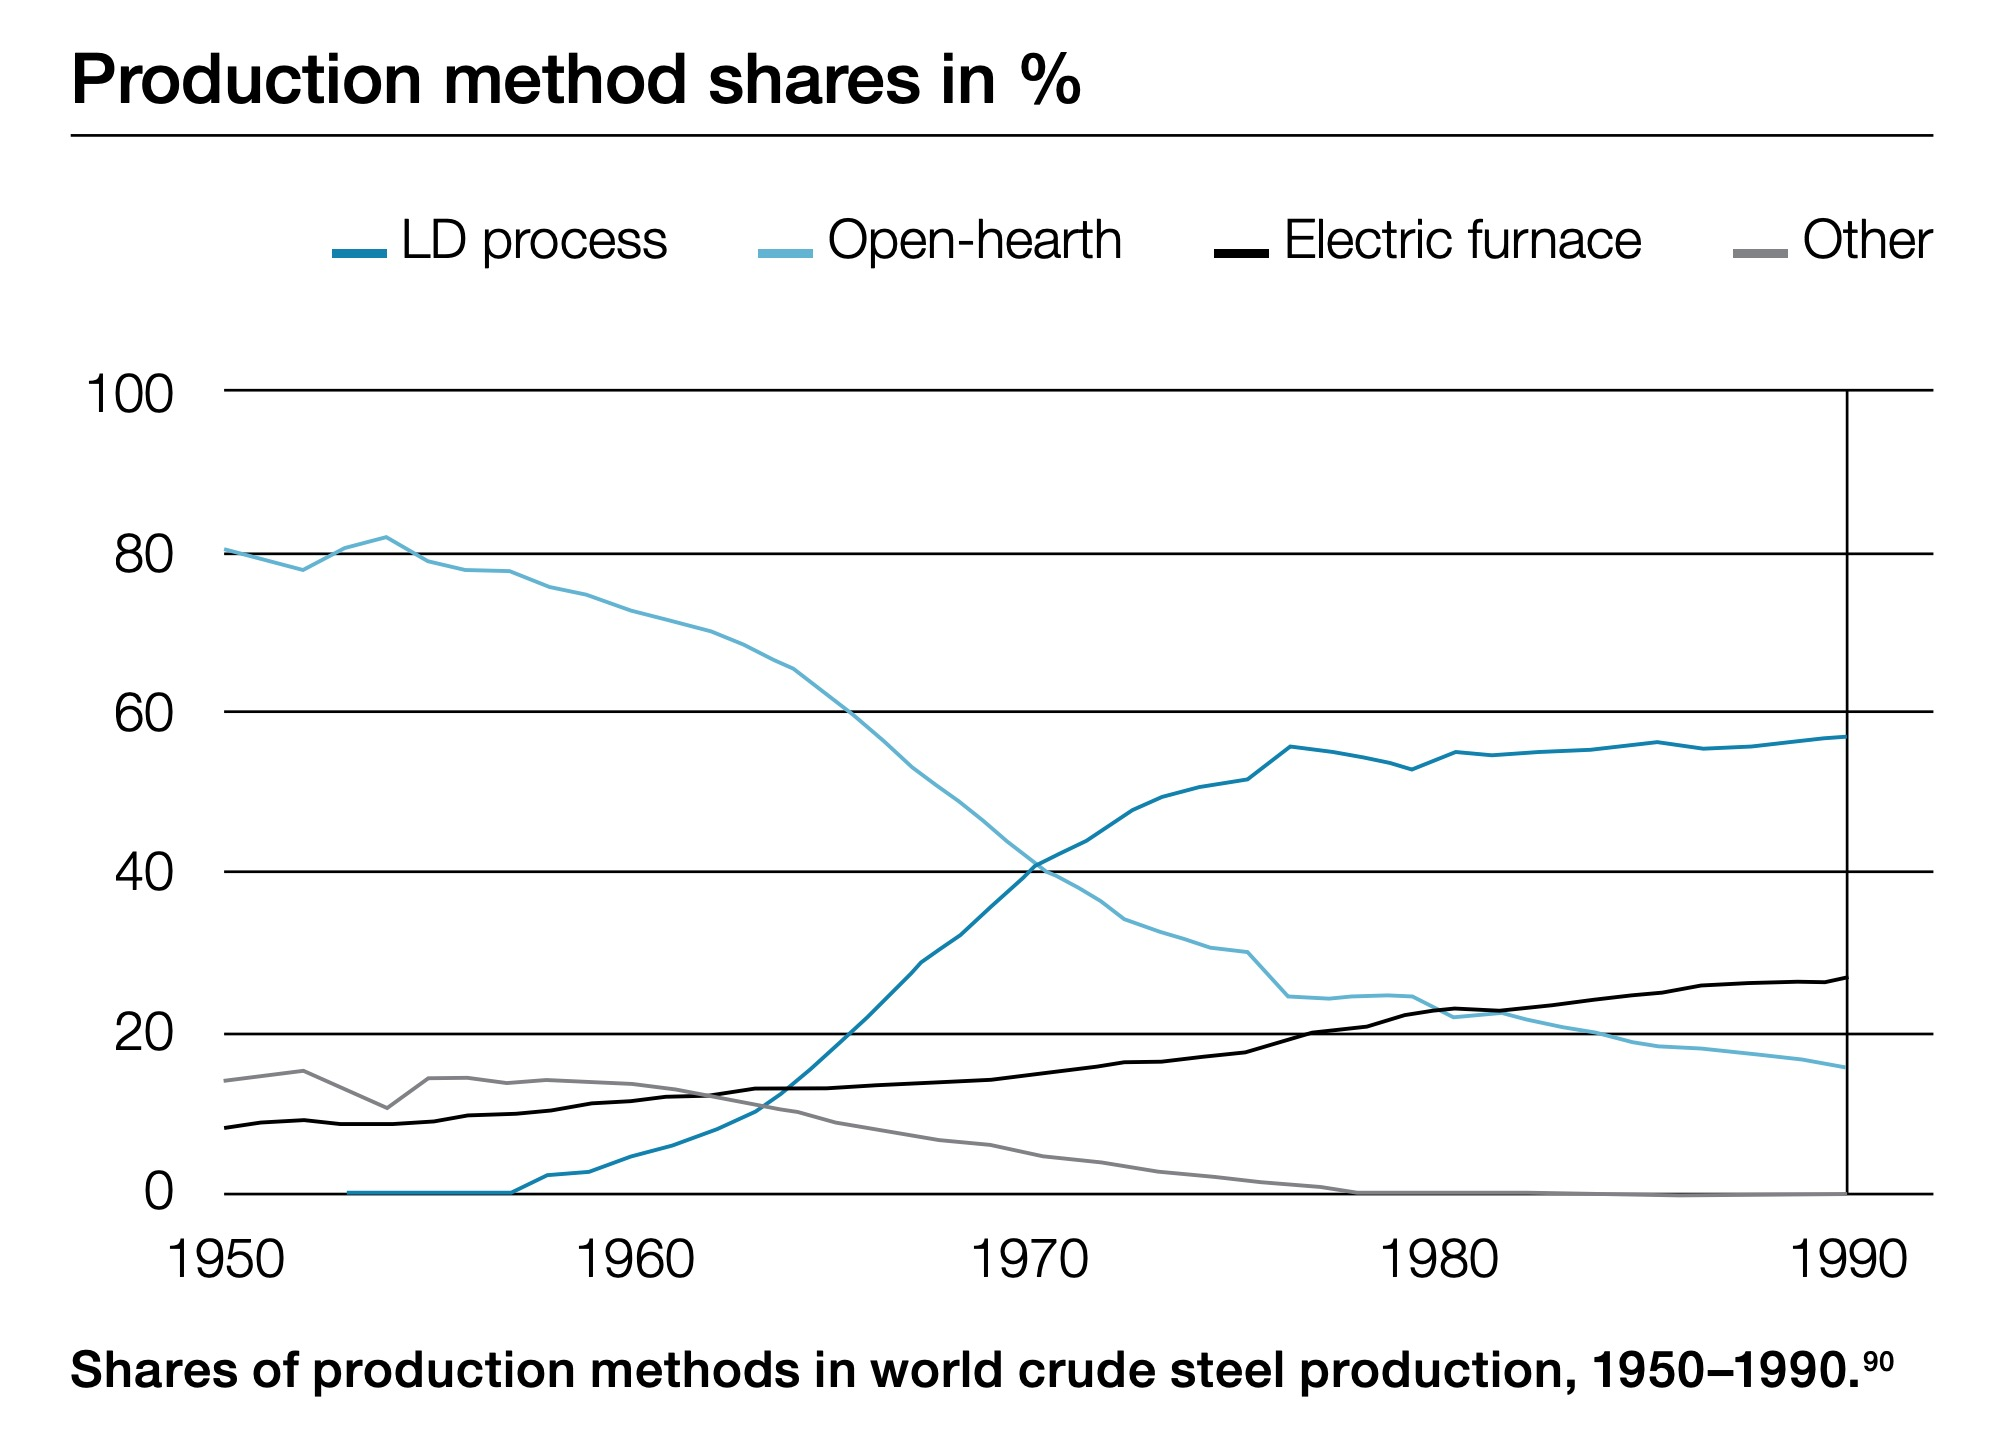
\includegraphics[width=.9\textwidth,angle=0]{ld-process-history-data.jpg}
\caption{Podiel výrobných medód ocele v percentách \citep{voestalpineLD2012}}
\label{o:1}
\end{figure}

Spomínaný LD proces sa v rôznych častiach sveta názýva odlišne. Napríklad vo Veľkej Británii sa označuje ako BOS (basic oxygen steelmaking); v Amerike a v Ázijských krajinách BOF (basix oxygen furnace) s výnimkou americkej korporácie U.S. Steel, kde sa často označuje ako BOP (basic oxygen process) \citep{Turkdogan1996}.

\begin{figure}
\centering
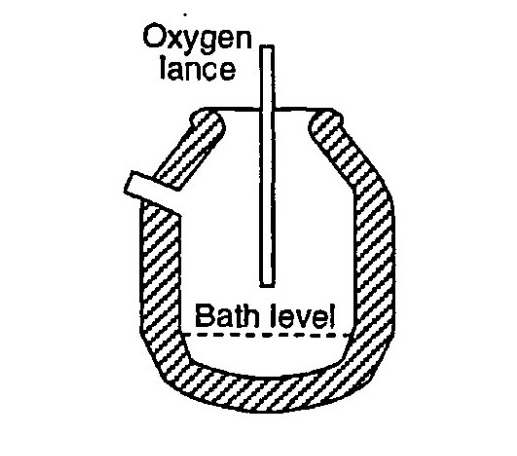
\includegraphics[width=.5\textwidth,angle=0]{bof-single.jpg}
\caption{Výroba ocele v konvertore fúkaním kyslíka zhora \citep{Turkdogan1996}.}
\label{o:2}
\end{figure}

V 70. rokoch bol v Kanade a Nemecku vyvinutý (a následne komercializovaný) upravený typ konvertora s vháňaním kyslíka z dolnej časti. Tento proces sa v Európe označuje ako OBM a v iných častiach sveta ako Q-BOP.

\begin{figure}
\centering
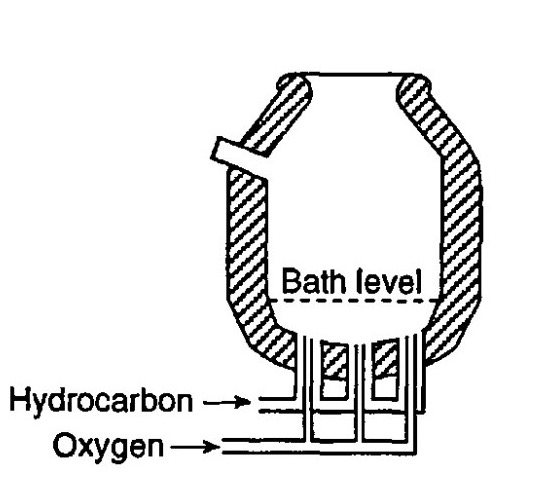
\includegraphics[width=.5\textwidth,angle=0]{q-bop.jpg}
\caption{Výroba ocele v konvertore fúkaním kyslíka zdola \citep{Turkdogan1996}.}
\label{o:3}
\end{figure}

V konvertore pre Q-BOP proces sa v dolnej časti nachádzajú trysky vsadené do odnímateľného dna, cez ktoré sú vháňané kyslík (\ce{O2}) spolu s páleným vápnom a prstencová medzera okolo centrálnej rúry na priechod plynného uhľovodíka (napr. propán alebo metán). Po kontakte s tekutou oceľou uhľovodík disociuje na \ce{C} a \ce{H2} pri absorpcii tepla. Táto endotermická reakcia potláča prehrievanie hrotu vyhadzovača exotermickou reakciou kyslíka s tekutou oceľou.

Ďalší vývojovým krokom výroby ocele v kyslíkovom konvertore bolo spojenie typov fúkania kyslíka zhora a zdola.


\begin{figure}[!tbp]
	\centering
	\subfloat[Kombinovaný BOF.]{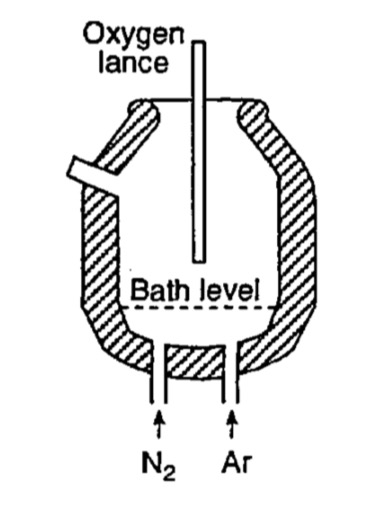
\includegraphics[width=0.38\textwidth]{kombinovany-bof.jpg}\label{fig:f1}}
	\hfill
	\subfloat[Kombinovaný Q-BOP.]{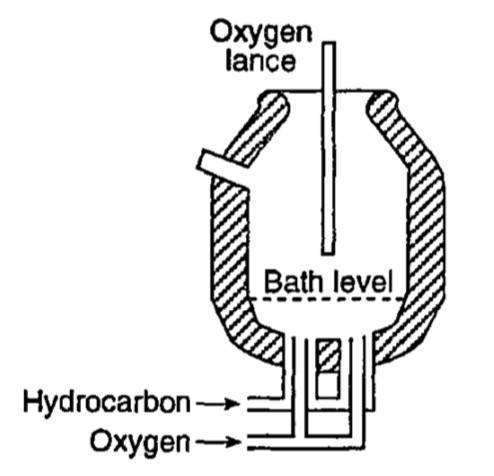
\includegraphics[width=0.52\textwidth]{kombinovany-q-bop.jpg}\label{fig:f2}}
	\caption{Výroba ocele procesom BOF a Q-BOP v LD konvertore s kombinovaným typom fúkania.}
	\label{o:4}
\end{figure}


-----------

Basic oxygen furnace (BOF) steelmaking is a complex process and dynamic model is very important for endpoint control. It is usually difficult to build a precise BOF endpoint dynamic model because many input variables affect the endpoint carbon content and temperature.


BOF is a widely preferred and effective steelmaking method
due to its high productivity and considerably low production cost. Therefore, almost 65\% of the total crude steel productions in the world are melted by using the BOF method. BOF steelmaking is a very complex chemical physical process. The quality of scrap iron changes from batch to batch. The grades of steel produced vary frequently, and the components of raw materials fluctuate largely \cite{Wang2010}.

The main objective of controlling oxygen converter steelmaking is to obtain prescribed parameters for the steel when it is tapped from the furnace, including weight, temperature, and each element content. In practical steelmaking process, the criterion whether the molten steel is acceptable or not is often decided by the endpoint carbon content and temperature.

-----------------------

Pri tejto metóde musí byť ale ešte dodávaná tavenina, aby dávka nevychladla.
Hotová oceľ sa potom vyleje z konvertora do panvy na ďalšie spracovanie.
Cenovo skoro najvýhodnejší spôsob výroby ocele pre veľké množstvá.

%
% !TeX encoding = UTF-8
% !TeX spellcheck = sk_SK
% !TeX root=teoriaprocesovtakac.tex
\section{Vstupy a výstupy}

Začnime rovnicou

\begin{equation}\label{r:2}
\frac{\ud^2y}{\ud t^2}+\frac{\ud y}{\ud t}+y =0, \qquad y(0)=1, \quad
y\,'(0)=15.
\end{equation}

Grafický priebeh riešenia tejto rovnice vidíme na Obrázku \ref{o:2}.

\begin{figure}[ht!]
\centering
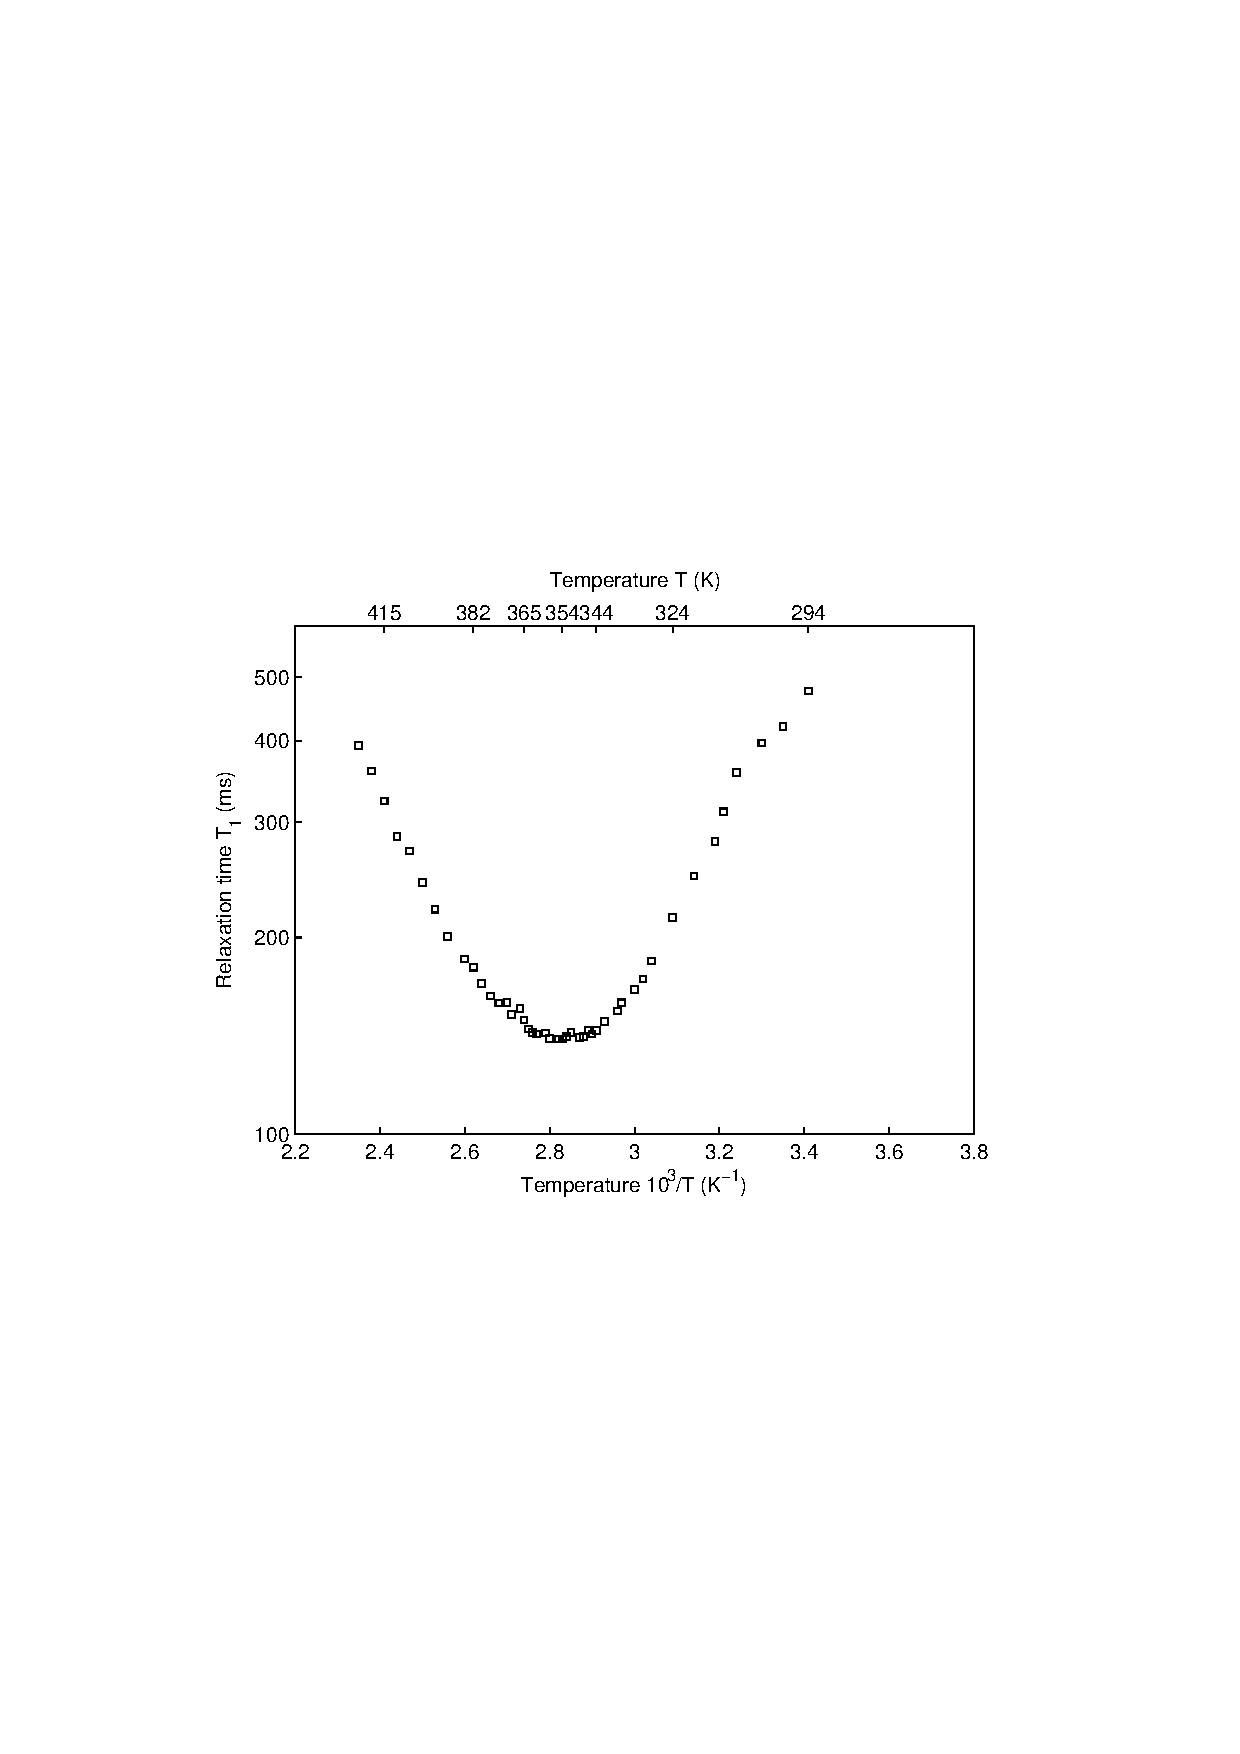
\includegraphics[width=.95\textwidth,angle=0]{relaxcas.pdf}
\caption{Teplotná závislosť spinovo-mriežkového relaxačného
času}\label{o:60}
\end{figure}

%\tabcolsep=3pt % sirka stlpcov
%\renewcommand{\arraystretch}{1.2} % riadkovanie
\begin{table}[ht!]
\centering
\caption{Parametre získané z~meraní spinovo-mriežkových relaxačných
časov $T_1$}\label{t:2}
\medskip
\newcolumntype{d}{D{,}{,}{-1}}
\begin{tabular}{||c||d|d|d|d|d||}
\hhline{|t:==t:==:==:t|}
\multicolumn{1}{||c||}{}&\multicolumn{1}{c|}{PP --
01}&\multicolumn{1}{c|}{PP -- 05}&\multicolumn{1}{c|}{PP --
10}&\multicolumn{1}{c|}{PP -- 16}&\multicolumn{1}{c||}{PP -- 22} \\
\hhline{|:==:==:==:|}
C $\cdot 10^8$~(s$^{-2}$) & 10,1 & 10,0 & 11,0 & 9,2 & 8  \\
\hhline{||-|-|-|-|-|-||}
$\tau_0 \cdot 10^{-14}$~(s) & 2,63 & 1,44 & 0,95 & 2,21 & 10,83  \\
\hhline{||-|-|-|-|-|-||}
$E_{\text a}$~(kJ) & 34,26 & 8,33 & 39,76 & 37,31 & 31,86  \\
\hhline{||-|-|-|-|-|-||}
$T_{\min}$~(K) & 354 & 367 & 367 & 369 & 367  \\
\hhline{||-|-|-|-|-|-||}
$T_{1\min}$~(ms) & 141 & 160 & 157 & 175 & 181  \\
\hhline{||-|-|-|-|-|-||}
$\Delta M_2$~(Gs$^2$) & 5,49 & 5,66 & 5,16 & 5,09 & 5,02  \\
\hhline{|b:==b:==:==:b|}
\end{tabular}
\end{table}


%
% !TeX root=teoriaprocesovtakac.tex
% !TeX encoding = UTF-8
% !TeX spellcheck = sk_SK
\section{Procesy v kyslíkovom konvertore}

Kroky, ktoré sú súčasťou LD procesu:

- Vsádzka (charging)

- Fúkanie (blowing)

- Vzorkovanie (sampling)

- Tapping

- Slag off


Cílem kyslíkové výroby oceli je spálení (tj. oxidace) nežádoucích nečistot obsažených v kovové vsázce. Hlavními prvky, které tudíž přecházejí na oxidy jsou uhlík, křemík, mangan, fosfor a síra.

Účelem tohoto oxidačního procesu tedy je :

snížit obsah uhlíku na předepsanou úroveň ( z přibližně 4\% na méně než 1 \%, ale často níže)
upravit obsah potřebných cizích prvků
odstranit nežádoucí nečistoty v maximálně možné míře
Výroba oceli kyslíkovým pochodem je diskontinuální proces, který zahrnuje následující kroky :

přepravu a skladování taveniny horkého kovu
předúpravu taveniny horkého kovu (odsiřování)
oxidaci v kyslíkovém konvertoru (oduhličení a oxidaci nečistot)
úpravu sekundární metalurgií
odlévání (kontinuální a/nebo do ingotů)


Podstatou výroby ocele v kyslíkovom konvertore je oxidácia prvkov z kovonosnej vsádzky s kyslíkom fúkaným do konvertora. Oxidy týchto prvkov prechádzajú do trosky alebo odchádzajú vo forme konvertorového plynu (Obr. 30). Intenzita oxidácie jednotlivých prvkov závisí od ich chemickej afinity ku kyslíku.
Oxidácia uhlíka je jedným z najdôležitejších procesov. Uhlík sa v kove počas
oceliarenského pochodu oxiduje vplyvom kyslíka najmä na \ce{CO} a čiastočne na \ce{CO2} podľa reakcií

\begin{equation}
\ce{C + 1/2O2 -> CO}
\end{equation}
\begin{equation}
\ce{C + O2 -> CO2}
\end{equation}

Mangán sa v konvertore oxiduje na \ce{MnO}

\begin{equation}
\ce{Mn + 1/2O2 -> MnO}
\end{equation}

Fosfor je v oceli nežiaduci a oxiduje sa na \ce{P2O5}

\begin{equation}
\ce{2P + 5/2O2 -> P2O5}
\end{equation}

Síra patrí medzi škodlivé prvky a prechádza do trosky vo forme \ce{CaS} na základe reakcie \ce{CaO}

\begin{equation}
\ce{CaO + MnS -> CaS + MnO}
\end{equation}

pričom \ce{MnS} vzniká podľa reakcie

\begin{equation}
\ce{Mn + S -> MnS}
\end{equation}

a síra taktiež odchádza aj vo forme plynu ako \ce{SO2}

\begin{equation}
\ce{S + O2 -> SO2}
\end{equation}

Kremík ma vysokú afinitu ku kyslíku, čiže sa ľahko oxiduje pričom vzniká \ce{SiO2}

\begin{equation}
\ce{Si + O2 -> SiO2}
\end{equation}

Potrebné je taktiež uvažovať aj straty železa vo forme \ce{FeO} a \ce{Fe2O3}

\begin{equation}
\ce{Fe + 1/2O2 -> FeO}
\end{equation}

\begin{equation}
\ce{2Fe + 3/2O2 -> Fe2O3}
\end{equation}

ktoré prechádzajú do trosky, resp. \ce{Fe2O3} odchádza v konvertorovom prachu. Kvapky kovového železa sa nachádzajú aj v troske (Obr. 30).


Vzniknutý SiO2 (29) prechádza do trosky ako \ce{2CaO.SiO2} podľa rovnice

\begin{equation}
\ce{SiO2 + 2CaO -> 2CaO.SiO2}
\end{equation}

a obdobne P2O5 (4) prechádza do trosky ako 3CaO.P2O5 podľa rovnice

\begin{equation}
\ce{P2O5 + 3CaO = 3CaO.P2O5}
\end{equation}


%
% !TeX encoding = UTF-8
% !TeX spellcheck = sk_SK
% !TeX root=teoriaprocesovtakac.tex
%%
\Urlmuskip=0mu plus 1mu\relax
\bibliographystyle{spbasic}
\bibliography{references}
%
\newpage
\phantomsection
\protect\label{page:posledna}

\end{document}
%%